\documentclass{llncs2e/llncs}
\usepackage{llncs2e/llncsdoc}

%\documentclass{sigchi/sigchi}

\usepackage{hyperref}
\usepackage{url}
\usepackage{graphics, graphicx}
\usepackage{caption}
\usepackage{csquotes}


\title{A Statistical Analysis of Adaptive Hints}

\author{Zhen Zhai\inst{1} \and Yoav Freund\inst{2}}
\institute{UC San Diego \email{zzhai@eng.ucsd.edu} \and UC San Diego \email{yfreund@eng.ucsd.edu}}

%\numberofauthors{2}
%author{
%  \alignauthor{Zhen Zhai\\
%    \affaddr{UC San Diego}\\
%    \email{zzhai@eng.ucsd.edu}}\\
%  \alignauthor{Yoav Freund\\
%    \affaddr{UC San Diego}\\
%    \email{yfreund@eng.ucsd.edu}}\\
%}

\begin{document}

\maketitle


%%%%%%%%%%%%%%%%%%%%%%%%%%%%%%%%%%%%%%%%%%%%%%%%%%%%%%%%%%%%%%%%%%%%%%%%%%%%%%%%
\begin{abstract}
We study the performance of an adaptive hint system we developed for
sending just-in-time feedback to students as they are working on
mathematical homework assignments.


We describe the system and the experimental design. Analysis of the
results demonstrate that hints improve learning. Specifically {\em a
  studet that recieves a hint when attempting to answer an assignment
  question will solve following quesions in the same assignment more
  quickly than a student that did not recieve the hint.}  On the other
hand, there was no significant correlation between the reception of
hints and the performance of the students in the final exam.

\end{abstract}


%%%%%%%%%%%%%%%%%%%%%%%%%%%%%%%%%%%%%%%%%%%%%%%%%%%%%%%%%%%%%%%%%%%%%%%%%%%%%%%%
\section{Introduction}
Intelligent tutoring systems (ITS)\cite{Anderson1995} attempt to replicate the interaction between a human tutor and a student. The goal is to detect and classify student errors and to provide instantaneous feedback to help students correct their error, but without "feeding" them the correct answer. Previous research suggests that a computer tutor can nearly be as effective as a human tutor\cite{Vanlehn2011}. Hence, many intelligent tutors have been developed and introduced into classrooms. A few well developed ITS designed for algebra curriculum in middle school and high school mathematics has already been proven to be effective\cite{Koedinger1997,John2014}.

Research has suggested that well-designed feedback is essential to improving the learning process\cite{Azevedo1995}\cite{Bangert-Drowns1991}. Formative feedback is feedback that aims to improve students learning and is presented in the form of a response to student incorrect answers\cite{Shute2008}. According to Shute~\cite{Shute2008}, formative feedback needs to be specific, clear and timely. Furthermore, formative feedback should provide learners with both verification and elaboration\cite{Mason2001}\cite{Bangert-Drowns1991}. Verification is to provide feedback to learners as to whether the answer is correct or not. Elaboration is to provide a short elaboration on the topic or discuss the learner's incorrect answer. The timing of the feedback is important as well, Kulhavy and Anderson suggest that delayed feedback is better than instance feedback\cite{Kulhavy1972}. The adaptive hint system delay hints by only providing hints to students who have spent a certain amount time on the problem without solving it. This allows the hints only go to students who are struggling with a problem. Finally, studies show that hint-on-demand allow students to learn more as compared to proactive hints\cite{Razzaq2010}. Therefore, the adaptive hint system is designed that a student will only see a hint if they click the 'Show Hint' button.

Homework is an essential part of students' learning process\cite{Cooper2006}. It gives students a chance to practice. Even more importantly, it allows them to identify their confusions and resolve them. There are many popular web-based homework systems for college students(e.g., WebAssign, WebWork, OWL, Andes). The goal is to help instructors to have a better management of a large enrollment class. These homework systems often provide feedback to students and provide analysis of student performance to instructors. Research has proven the web-based homework(WBH) systems to be helpful in learning\cite{MestHartRath2002}\cite{Vanlehn2005}. In these studies, the WBH systems, OWL and Andes, provide students with immediate feedback and hints following an incorrect attempt\cite{MestHartRath2002}\cite{Vanlehn2005}. The feedback and hints are the essential part of a WBH system, which is what our study focuses on.

\cite{ElkherjFreund14} described a system for delivering hints in the context of a web-based homework system. In the work presented here, we describe a controlled experiment that we have done in the context of an undergraduate course in probability and statistics. Our statical analysis provides new evidence that adaptive hints are effective.

There is a common concern about students gaming the system, especially on harmful gaming, where gaming the system leads to poor learning outcome\cite{Baker2004}\cite{Baker2005}. In previous studies, students game the system by tricking the tutoring systems into giving out correct answers\cite{Baker2004Off-task}. As a result, students succeed in homework but fail on learning. We don't have this concern because our hints don't contain correct answers in any form. The adaptive hint system generates short simple questions as hints instead of worked-examples, which is commonly used among human tutors\cite{Atkinson2000}. In fact, it is suggested that worked examples have no significant effects on learning in a web-based intelligent tutoring environment\cite{McLaren2006}. Therefore, we replaced worked examples with short questions that are designed to promote thinking and guide student's learning process. This resolve the concern of students gaming the system because our system gives students hints on how to learn instead of how to answer a specific question. The only way for a student to obtain correct answers is by learning how to solve the problem. Therefore, we not only prevent any system gaming, but our hints also help students in long term. Furthermore, our hint system targets mathematic problems, which require students to type in mathematic expressions. Therefore, unlike multiple choice problems, it would be nearly impossible to guess the answer by looking at hints. There is infinity many ways one can type in a mathematic expression and it is very hard for students to simply guess it correctly with the help of hints. Therefore, we don't have the concern of students gaming the system.

\subsection*{Contribution}
We built and implemented an adaptive hint system to provide hints to students at the time they are struggling with homework. The adaptive hint system first studies a student's incorrect answer to identify the student's confusion. We target mathematics problems that require students to type in an expression, therefore the system generates a message to point out the incorrect subexpression in a student's answer. Then, based on the identified confusion, the system explains the identified confusion with a short sentence followed by a short question for the student to solve. This short question is specifically designed to target the student's confusion and it is simple enough that a student can easily understand and answer. Our goal is to let the student solve the smaller task before moving on to solve the bigger task. The goal of the adaptive hint system is to guides students in their learning process from understanding their confusions to resolve their confusions.

The system is adopted in a probability and statistic class of around 300 students and 245 students participated in this research. Each week we assign one assignment to students and we sent hints from the fourth week to the eighth week of the quarter. There are a total of 26 problems and each problem has between 1 to 10 questions. According to our record, students have received a total of 3621 hints during these five weeks. Our statistical result shows that students, with the help of the adaptive hints, learn to solve the problem and can solve similar problems more efficiently afterward. Our analysis demonstrates with statistical significant less than $1\%$ that students who receive a hint spent fewer attempts and also less amount of time on later problems in the same assignment compared to students who didn't receive a hint.


\section{The Adaptive Hint System}
The adaptive hint system is built on top of Open edX, an open source MOOC platform. We used Open edX as our homework system and embedded our adaptive hint system on top of Open edX. The edX homework system prompts students to answer problems by entering mathematical expressions and provides instant feedback on the correctness of the answer. The adaptive hint system provides additional feedback in the form of a hint. Students receive one assignment per week. Each assignment contains 5 to 10 problems and each problem has 1 to 10 parts. The problems in an assignment all target similar material that is covered in lecture. Students have an unlimited number of attempts for each problem, they can spend as many attempts as they want until they get to the correct answer.

Our adaptive hint system is built by creating hints beforehand based on historical data. After we release the homework, the hint system starts to parse student attempts to figure out students' confusion. Then it looks for the appropriate hint in the hint database and sends to students.


\subsection*{Creating Hints}

Hints are created before we release the homework assignments. This allows the system to have a pool of hints to start with at the time the assignment is released. To create useful hints, the teaching staff analyzes the incorrect student attempts from previous quarters and create hints accordingly. The hints created are consist of a short explanation followed by a short question for the student to answer.

For example, one question would be "How many strings contain $k$ digits and $j$ uppercase letters?". The correct answer is $10^k*26^j*C(k+j,k)$. Suppose a student answers $10^k*26^j*(k+j)!$, the system would identify the incorrect subexpression and generate the following hint

\begin{displayquote}
The subexpression $10^k*26^j$ is correct, but not $(k+j)!$. How many ways are there to arrange 2 digits and 1 letter?
\end{displayquote}


This way we encourage students to focus on the incorrect part of their answers and solve a simpler version of it before attempting to solve the original problem. Moreover, as the hint is given in the form of a question, we guide the student to think about the same problem in a simplified setting and leave it to them to infer the correct answer to the original problem. Note that students can choose to answer or not answer these hint questions. If students choose to answer the hint questions, we will provide instant feedback to let the students know whether their answers are correct or not. If students choose not to answer the hint questions, it won't hurt their grade.

Other than the problem specific hints, we also have generic hints. For example, when a student types in a number instead of an expression, our system will send a hint telling the student to type in an expression instead of the calculated result. Another example would be a hint pointing out that the question is asking for a positive number but the student typed in a negative number. These generic hints are designed to point out some very general mistakes students tend to make in a probability and statistics class. The system tends to send the generic hint before sending the specific hint.


\subsection*{Parse Trees}
The adaptive hint system needs to parse student attempts. Since we are targeting math expression problems, we can use parse trees to parse the math expressions. The parse tree always has operators as tree parents and operands as children. See Fig. \ref{fig:parse_tree}. Each tree node is marked by its position in the tree. The root node is node $R$. The left child node is indicated by $0$ and right child is $1$. Therefore, the left tree node of node $R$ is $R.0$, and right node is $R.1$. 

\begin{figure}[ht]
   \centering
   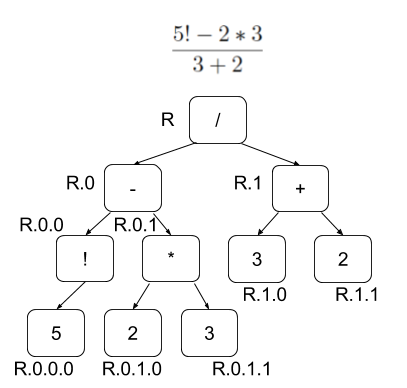
\includegraphics[width=.5\textwidth]{image/Parse_Trees.png}
   \caption{The parse tree mark each tree node by position. "R" stands for root node, "0" stands for left child node and "1" stands for right child node. Therefore, "R.0.1" stands for the right child node of the root's left child.}
   \label{fig:parse_tree}
\end{figure}

To figure out the mistake in an attempt, we compare the parse tree of the attempt with the parse tree of the correct answer. The tree comparison can tell us the subexpression that students make mistakes on. We can then classify student inputs based on the incorrect subexpressions and assign hints correspondingly. For example, the student who typed $5!-2*3$ and the student who typed $\frac{5!-2*3}{10}$ for a problem with solution $\frac{5!-2*3}{3+2}$, as in Fig. \ref{fig:parse_tree}, would be classified as the same group. Both of the students will have a mismatch of tree node $R.1$. This tells the system that the subtree of $R.1$ is wrong and the system will look for the corresponding hint.

One problem is that there are many different ways to write the same math expression. For example, $5!$ can also be written as $5*4*3*2*1$ or $5*4*3*2$. Therefore, we evaluate each subtree to a numerical result and use it in our comparison. The parse trees are evaluated bottom up. The operators at the bottom of the trees are evaluated first. The root operator is evaluated last. See Fig. \ref{fig:eval_tree}. 

\begin{figure}[ht]
   \centering
   \caption{The parse tree is evaluated bottom up. We first evaluate the lowest level of the tree then pass the evaluated results to the upper level. Then use the lower level results to evaluate the upper level of the tree until we reach the top node of the tree, the root, which will give us the final numerical result of the expression.}
   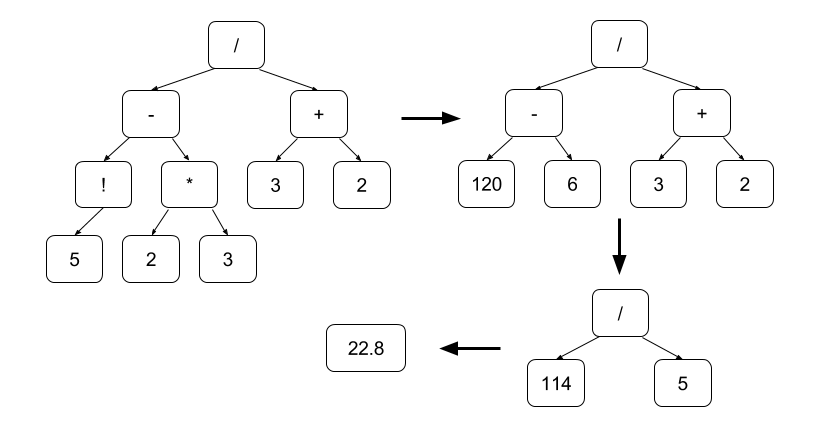
\includegraphics[width=0.8\textwidth]{image/Eval_Trees.png}
   \label{fig:eval_tree}
\end{figure}

Both the parse tree and the evaluation tree are used when we compare the attempt to the correct answer. We identify a subtree as incorrect only when neither of the evaluation and the subtree doesn't match. Therefore, $5!$ and $5*4*3*2*1$ will be identified as the same subtree because it evaluates to the same result.


\subsection*{Assigning Hints}
When TAs create hints, they are also asked to specify rules. Hint rules tell the system when to send certain hints and who the hints will go to. One example of hint rule for expression in Fig. \ref{fig:parse_tree} could be "$R.0.0$ is wrong" and the corresponding hint could be "You need to find the number of ways to arrange different poker cards. How many ways can you arrange 2 different cards?". When the hint system captures an attempt with an incorrect $R.0.0$ subtree, this hint will be sent. Such attempts could be $\frac{4!-2*3}{3+2}$ or $\frac{30-2*3}{3+2}$. The adaptive hint system will assign hints automatically based on the hint rules. This allows our hints to be sent automatically.

Note that the system doesn't send hints to the student right away. Hints are only sent to students who have been working on the problem for more than 5 minutes or students who did more than 3 attempts. This is how the system sends delayed hint suggested by Kulhavy and Anderson\cite{Kulhavy1972}. This way hints only go to students who are working on the problem actively and are struggling. Furthermore, students need to demand hints by clicking the "Show Hints" button. Hint-on-demand is suggested to be more effective than proactive hints\cite{Razzaq2010}. Once a hint is assigned to a student, the student can choose to click or not click the "Show Hint" button. One can ignore the assigned hint by not clicking the "Show Hint" button. If a student wants to see the assigned hint, he/she needs to click the "Show Hint" button to see the hint. See Fig. \ref{fig:show_hint} In other words, we only show hints to students who ask for hints. Students who don't click the "Show Hints" button will not see the assigned hints. This makes sure we give on-demand hints to students who need helps and actively ask for help. 

\begin{figure}[ht]
   \centering
   \caption{First the system decides whether to assign hints to a student. Then the system search through the hint database to see whether there is a hint condition satisfied. Finally, the student gets to decide whether to see the assigned hint. A student will see a hint only if the system decides to assign the hint, a hint condition is satisfied, and the student clicked the ``Show Hint'' button.}
   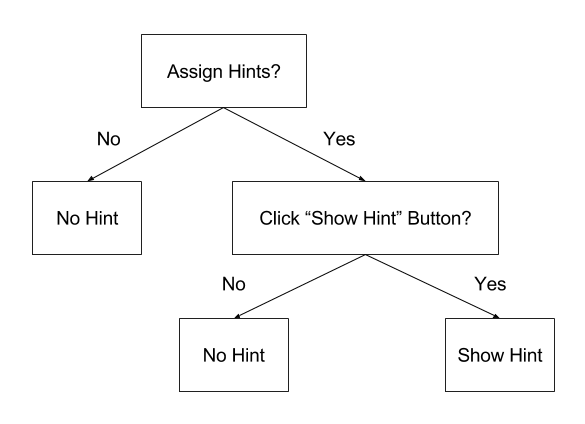
\includegraphics[width=0.7\textwidth]{image/Show_Hint.png}
   \label{fig:show_hint}
\end{figure}


\section{Statistical Study of the Effectiveness of hints}

We used a controlled study to quantify the effect of our hints on
student performance. For four of the weekly assignments, we randomly
placed each student with equal odds into a case group or a control
group. We refer to those students as case students and control
students.  We use the term {\em session} to refer to the record of a
single student working on a single problem. We use the term {\em
  attempt} to refer to a single attempted answer a student sends to
the edX system.

We filter out case student sessions in which the student did not
receive a hint, either because her attempt did not trigger a hint or
because she did not click on the ``show hint'' button.  To make the
control set as similar as possible, we filter out Control student
sessions whose attempts would not have triggered a hint had they been
in the case set.

To quantify the effect we use three measures:
\begin{itemize}
\item {\bf Number of attempts:} Students were given an unlimited number of attempts. In most cases, students made attempts until they found a correct answer. We use the number of attempts to quantify the degree of difficulty experienced by the student when solving the problem.

\item {\bf Total attempt time:} In addition to the number of attempts, we estimate the total amount of time the student spent on the problem. Students periodically take a break and continue after a few hours or days, we reduce the effect of such time gaps on our estimate by eliminating any time gap longer than ten minutes.
\item {\bf Problem grade in final:} Most homework assignments have a corresonding problem in the final exam. We use the grade of said problem to quantify the long-term effect of receiving hints. 
\end{itemize}

Our goal is to establish that the hints we produce have a positive
effect on learning. The null hypothesis that we aim to reject is that
hints have no effect. We consider the potential effect at three
different time scales. The {\em within problem effect} is the effect
of receiving a hint when attempting to answer a problem on the
performance of the student {\em on the same problem}. The {\em within
  assignment effect} is the effect of receiving a hint when attempting
to solve a problem on the performance of the students on later problem
{\em within the same assignment}. Finally, the {\em long-term effect}
is the effect of receiving hints during an assignment on the
performance of the student on questions on the same material in the
final exam.

We found no statistically significant effect for either the within problem or
the long-term effect. On the other hand, we found a significant effect
on the same assignment. We present the analysis and then discuss.

\subsection{Within problem effect}

Our first attempt was to evaluate whether receiving a hint while
working on a problem helps the student solve the problem faster than
otherwise.

We consider each problem within the four weeks of our evaluation. For
each problem we compute the number of attempts and the length of time
each student spent on the problem. We compare the number of attempts
and the length of time for each problem between the case students who
received at least one hint and the control students
that would have recieved a hint were they in the case group.

The results are summarized in
Figure~\ref{fig:tries_times_analysis}. Application of a t-test fails
to detect a difference between the case and the control.

\iffalse
We also extract the time students spent on each problem. We measure the time differences between each attempt and filter time gaps that are longer than 10 minutes. Time gaps larger than 10 minutes are considered as a break instead of time spent on homework. Then we sum up all the time gaps between attempts as the total time a student spent on the problem. We again compare average time spent of case students with control students, see the graph on the right of Fig. \ref{fig:tries_times_analysis}. The graph of the number of attempts is consistent with the graph of time spent. We can't detect the effectiveness of hints on the problems where students receive and read hints and try to do the short questions in hints. Note that students who received hints are likely to spend more time on these problems because all our hints are short questions designed for students to answer. Students will likely to spend the time to read and do the hint questions.

\fi
\begin{figure}[ht]
\centering
   \begin{tabular}{c c}
		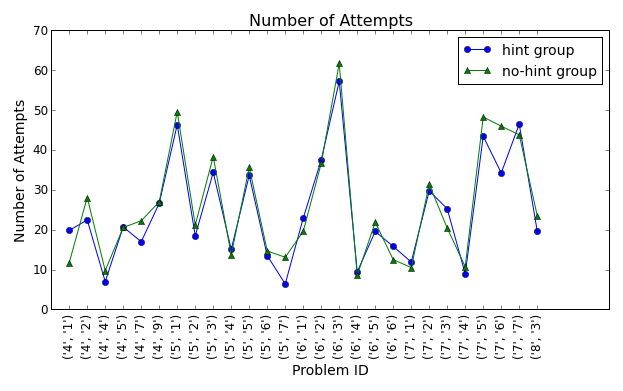
\includegraphics[width=0.5\textwidth]{image/new_tries_analysis.png} &
		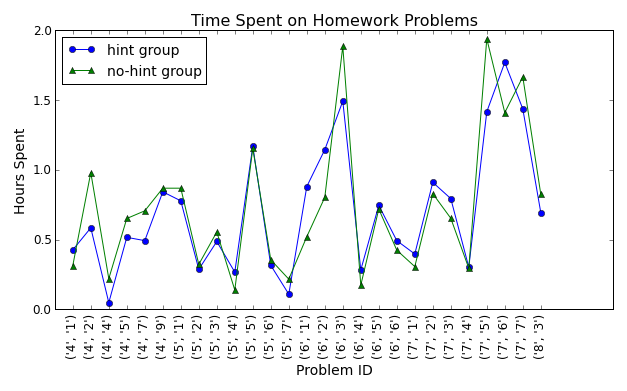
\includegraphics[width=0.5\textwidth]{image/new_times_analysis.png}
	\end{tabular}
\caption{On the left, the graph shows number of attempts for each problem average over control students vs case students. These problems are problems that at least one student received hints on. It shows that case students who ask for hints spent more attempts on these problems than the control students. On the right is the graph of time spent on each problem average over control students vs case students. Case students again spend more time on problems than the control students. Both graphs produce consistent results.}
    \label{fig:tries_times_analysis}
\end{figure}

\subsection{Within assignment effect}

Our second attempt was to evaluate whether receiving a hint while
working on an assignment helps the student solve a later problem faster
than otherwise.

We define ``problem with hint'' as follows. For the case student, a
problem with hint is a problem where a hint was sent to the student
who then chose to view it. For a control student, it is a problem for
which a hint would have been sent, had the student been in the case.

We consider only sessions that have at least one problem with
hint. For each such session, we consider all of the problems {\em
  without hint} that the student worked on after working on the
problem with hint. We call these problems the ``downstream'' problems.

For example, suppose the student solved an assignment of 9 problems in the
following order $\{ 1, 4, 3, 2, 6, 5, 7, 8, 9\}$. This student
received at least one hint on problems $\{3, 5, 7\}$. Therefore, the
downstream problems for this session are $\{2, 6, 8, 9\}$. See
Figure~\ref{fig:pro_no_hint}.

For each session, we compute the number of attempts (and the amount of
time) spent on each of the downstream problems. We partition these
measurements into two population depending on whether the student was
in the case or the control.

{\bf Yoav:} Zhen, I am confused about how you combined the information
from the different problems in an assignment. for each problem we have
two sets of numbers - one for the case, and one for the control. The
sizes of the two sets varies depending on when the hints were
given. If you were comparing one problem at a time, then a
two-population t-test can be used. But you are using something like
the total number of attempts for all of the problems in the
assignment... not sure how you are doing that. What are you summing?
{\bf Zhen:} I included the detail here https://www.overleaf.com/13310110vzkywdhhmcxd

For each student in case, we compute the number of attempts (or the length of time) for all downstream problems and aggregate the measurement for each assignment. On the other hand, we sum the average number of attempts( or the length of time) of control group for these same downstream problems. As a result, we have a sum of attempts (or time) and also an average of attemtps(or time) for each case student in each assignment. We compare the average of attemtps (or the length of time) on each assignment between control students and case students. See Fig \ref{fig:downstream_analysis}, both graphs show that students in the case group spent less attempts and also less amount of time on homework problems comparing to control students.

We then perform a one sample t-test with null hypothesis that the mean of the sum of attempts is the same as the average of attemtps. Table \ref{tab:no_hint} and Table \ref{tab:no_hint_time} show that we have small p-value for each of the assignment for both analysis of attempts and time. Therefore, we reject the null hypothesis and conclude that case students and control students have significantly different performance. This analysis shows that the adaptive hint system helps students to learn to solve similar problems that come later in the assignment. 

\begin{figure}[ht]
   \centering
   \caption{We filter out the problems that come before the first problem with hints. We only look at problems that come after problem 3 in the above example. We then sum up the attempts and compare the sum of attempts for student A and our baseline.}
   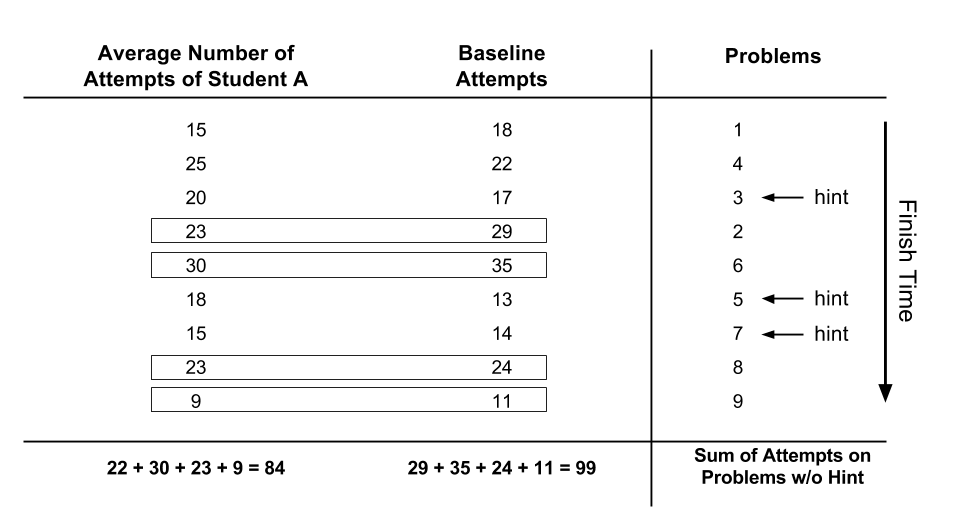
\includegraphics[width=0.8\textwidth]{image/Filter_problems.png}
   \label{fig:pro_no_hint}
\end{figure}

\begin{table}[th]
\caption{The table listed the extra number of attempts that control students spent comparing to case students. For the each of the four weeks, the control students spent more attempts than the case students. We also perform a one sample t-test with the null hypothesis that control students should have the same amount of attempts on problems as case students. The final p-value of the one sample t-test for all assignments is small enough that we can reject the null hypothesis.}
\begin{center}
  \begin{tabular}{| c | c | c | c | c | c |}
  \hline
    Week & Size of & Mean of & Std of &  P-Value of & Extra Attempts \\
    Number & Case & Attempts in Case & Attempts in Case & Two-Tail T-Test & Control Spent  \\ \hline
	4 & 43 & 47.674 & 23.125 & $0.000146$ & 22.235\\
	5 & 81 & 32.691 & 25.924 & $3.723 * 10 ^{-14}$ & 43.128\\
	6 & 64 & 47.438 & 37.967 & $0.00232$ & 19.956 \\
	7 & 55 & 93.636 & 37.451 & $1.3101 * 10^{-16}$ & 86.785\\
	\hline
  \end{tabular}
  \label{tab:no_hint}
  \end{center}
\end{table}

\begin{table}
\caption{The table listed the extra minutes that control spent comparing to case. We first compare the time spent for each assignment, then we look at all assignments at the end. We perform a two tailed t-test with the null hypothesis that control students spent the same amount of time on problems as case students. The final p-value of the two tailed t-test for all assignments is small enough that we can reject the null hypothesis.}
\begin{center}
  \begin{tabular}{| c | c | c | c | c | c |}
    \hline
    Week & Size of & Mean of & Std of &  P-Value of & Extra Minutes \\
    Number & Case & Minutes in Case & Minutes in Case & Two-Tail T-Test & Control Spent  \\ \hline
	4 & 41 & 81.141 & 48.998 & 0.168 & 13.885\\
	5 & 62 & 32.155 & 32.006 & $1.517 * 10^{-6}$ & 33.158\\
	6 & 58 & 73.519 & 77.389 & 0.0609 & 23.281 \\
	7 & 53 & 140.654 & 97.816 & $1.72 * 10^{-5}$ & 90.636 \\
	\hline
  \end{tabular}
  \label{tab:no_hint_time}
  \end{center}
\end{table}

\begin{figure}[ht]
\centering
   \begin{tabular}{c c}
		
\includegraphics[width=0.5\textwidth]{image/assignment_tries_downstream.png} &
		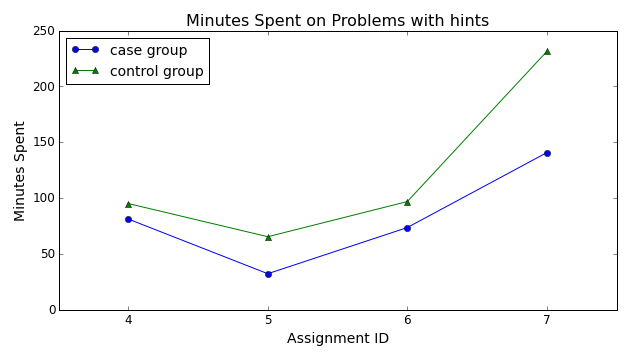
\includegraphics[width=0.5\textwidth]{image/assignment_time_downstream.png}
	\end{tabular}
\caption{On the left, the graph shows number of attempts for both control students and case student. The control students spent more attempts on each assignment comparing to the case students. On the right is the graph of time spent on each problem of control students and case students. Control students again spend more time on each assignment than the control students. Both graphs produce consistent results that adaptive hints improve students' homework performance.}
    \label{fig:downstream_analysis}
\end{figure}




\subsection{Long term effect}
Final scores play an important role as to evaluate the learning outcome of students. We examine whether hints have effect on students' final score.

The problems in the final exam aim to examine students understanding of different topics learned throughout the college quarter. Each of these topics have a collection of homework problems for students to practice. Therefore, we select a set of homework problems for each of the final problem as shown in Table \ref{tab:map}.

\begin{table}[h]
\caption{Each final problem on the left has a set of corresponding homework problems on the right. The problem ID is in the format of week number and problem number. For example, (4,1) means problem 1 of week 4 assignment.}
\begin{center}
  \begin{tabular}{ c | c }
   Final Problem & Homework Problem IDs \\ \hline
	3 & (4,1), (4,2) \\
	4 & (5,1), (5,2), (5,3), (5,4) \\
    5 & (6,4) \\
    6 & (6,6) \\
    7 & (6,2), (6,3) \\
    8 & (8,3), (8,4), (8,5), (8,6) \\ \hline
  \end{tabular}
  \label{tab:map}
  \end{center}
\end{table}

For each final problem, we look at the corresponding assignment. The control and case students of the corresponding assignment will then be the control and case students of the final problem. We compare control and case students on their final score for each final problem. See Figure \ref{fig:final_compare_all}.

\begin{figure}[h]
\centering
\caption{The graph shows average final scores of each final problem. The data points are labeled with p-value of a two-tailed t-test. We don't see a very clear advantage on either of the control or case.}
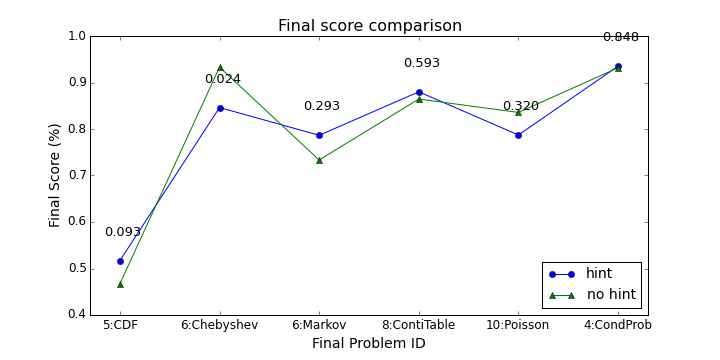
\includegraphics[width=0.8\linewidth, height=5cm]{image/final_compare.png}
\label{fig:final_compare_all}
\end{figure}

We can't tell which group of students perform better than the other. The p-values are not small enough and we conclude that the effect of hints on final scores is non-detectable.


\section{Conclusion}
We built an adaptive hint system for mathematics problems that can be embedded on any web-based homework platform. The system provides students with on-demand formative feedback to guide their learning process to achieve better learning outcome. Although we can't detect an improved in the final exam, our statistics show an improvement of students' performance on homework. We show that students with the help of the adaptive hints spent less time and less attempts on homework problems compared to students without the help of hints.

\newpage
\bibliographystyle{splncs}
\bibliography{bibtxt}



\end{document}
